\documentclass[aspectratio=169]{beamer}
\usepackage{amsmath}
\usepackage{amssymb}
\usepackage{tikz}
\usepackage{wasysym}
\usepackage{tikzsymbols}
\usepackage{xcolor}
\usepackage{animate}     % Option 1: play a PNG frame sequence
\usepackage{multimedia}  % Option 2: embed a video file (needs -shell-escape)
\usetikzlibrary{shapes,backgrounds,patterns}

% --- added for these slides -------------------------------------------------
\usepackage{pgfplots}
\pgfplotsset{compat=1.18, legend cell align=left}
\usetikzlibrary{arrows.meta,decorations.pathreplacing,calc,positioning}
\usepackage{listings}
\usepackage{booktabs}
\usepackage{array}
% ----------------------------------------------------------------------------

% royalblue isn't a base xcolor name, so define it first (this is the default accent)
\definecolor{royalblue}{RGB}{65,105,225}

% ============================================================
%  ACCENT COLOR: change ONE line below to switch the theme
%  Choose one of: royalblue , red , black
% ============================================================
\colorlet{accent}{royalblue}
% \colorlet{accent}{red}
% \colorlet{accent}{black}
% ============================================================

% Use default theme with white background
\usetheme{default}

% Make everything white/black, with the chosen accent color for structure
\setbeamercolor{background canvas}{bg=white}
\setbeamercolor{normal text}{fg=black}
\setbeamercolor{structure}{fg=accent}
\setbeamercolor{frametitle}{fg=accent,bg=white}
\setbeamercolor{title}{fg=accent}
\setbeamercolor{section in toc}{fg=black}
\setbeamercolor{block title}{fg=black,bg=gray!10}
\setbeamercolor{block body}{fg=black,bg=gray!5}
\setbeamercolor{block title example}{fg=black,bg=green!10}
\setbeamercolor{block body example}{fg=black,bg=green!5}
\setbeamercolor{block title alerted}{fg=black,bg=red!10}
\setbeamercolor{block body alerted}{fg=black,bg=red!5}

\usepackage{scalerel}

\newcommand{\subsmall}[1]{_{\scaleto{#1}{4pt}}}
\newcommand{\supsmall}[1]{^{\scaleto{#1}{2pt}}}

% Remove navigation symbols
\setbeamertemplate{navigation symbols}{}

% Simple footline with page numbers (single definition)
\setbeamertemplate{footline}{
    \hfill\makebox[5pt]{%
        \scriptsize\insertframenumber}
    \hspace*{2em}
    \vspace{0.5cm}
}

% Custom command for colored boxes
\newcommand{\cbox}[2]{\colorbox{#1}{\ensuremath{\displaystyle #2}}}

% --- code listings (Python), coloured with the accent -----------------------
\lstdefinestyle{py}{
  language=Python,
  basicstyle=\ttfamily\footnotesize,
  keywordstyle=\color{accent}\bfseries,
  commentstyle=\color{gray}\itshape,
  stringstyle=\color{green!45!black},
  showstringspaces=false,
  columns=fullflexible,
  keepspaces=true,
  backgroundcolor=\color{gray!6},
  frame=single, rulecolor=\color{gray!30},
  xleftmargin=2pt, xrightmargin=2pt,
  escapeinside={(*}{*)}
}
\lstset{style=py}

% --- shared plot style for the three "bound" pictures ------------------------
\pgfplotsset{
  boundplot/.style={
    width=5.9cm, height=4.6cm,
    axis lines=left, xmin=0, xmax=10, ymin=0, ymax=12,
    xtick=\empty, ytick=\empty,
    xlabel={$n$}, ylabel={time},
    every axis x label/.style={at={(axis description cs:1,0)},anchor=north east},
    every axis y label/.style={at={(axis description cs:0,1)},anchor=south east},
    samples=160, thick, clip mode=individual
  }
}

\title{Asymptotic Notation \& Convergence of Algorithms}
\subtitle{Review of complexity and floating point, then analysis of algorithms}
\author{Sharareh Sayyad}
\institute{Washington state University}
\date{September 28, 2026}

\begin{document}

\frame{\titlepage}

\begin{frame}{Outline}
\tableofcontents
\end{frame}

% ============================================================
\section{Review: complexity and floating point}
% ============================================================

\begin{frame}{Review of last session}
\begin{columns}[T]
\begin{column}{0.44\textwidth}
\begin{block}{Computational complexity}
\small
\begin{itemize}
  \item The resources an algorithm needs, as a function of the input size $n$.
  \item \textbf{Time}: number of \textbf{flops} ($+,-,\times,\div$ on floats).
  \item \textbf{Space}: extra memory beyond the input.
\end{itemize}
\end{block}
\end{column}
\begin{column}{0.53\textwidth}
\begin{block}{Floating point}
\small
\begin{itemize}
  \item Scientific notation in base 2: 64 bits (1 sign, 11 exponent, 52 fraction).
  \item $\varepsilon = 2^{-52} \approx 2.2\times10^{-16}$: about 16 significant digits; every flop is rounded.
  \item Gaps grow with size: $2.2\times10^{-16}$ near $1$, but $2$ near $10^{16}$.
\end{itemize}
\end{block}
\begin{alertblock}{Pitfalls}
\footnotesize never test floats with \texttt{==}; small $+$ large loses the small; subtracting nearly equal numbers destroys digits.
\end{alertblock}
\end{column}
\end{columns}
\vspace{0.2cm}
\centering\scriptsize Today: \textbf{Big-$O$} makes ``how the time grows'' precise, and \textbf{convergence} meets the floating point floor of $10^{-16}$.
\end{frame}

% ============================================================
\section{Big-$O$ notation}
% ============================================================

\begin{frame}{Big-$O$: what it tells you}
\begin{columns}[c]
\begin{column}{0.55\textwidth}
\small
\begin{block}{}
\centering \textbf{If the input gets bigger, roughly how much more work is needed?}\\
\scriptsize (for large inputs, ignoring constant factors such as a faster computer)
\end{block}
\begin{block}{Definition}
$f = O(g)$ as $x \to \infty$ if there are constants $c > 0$ and $x_0 \ge 0$ with
\[ |f(x)| \le c\, g(x) \quad \text{for all } x \ge x_0. \]
\end{block}
\scriptsize In words: from some point $x_0$ on, $f$ never exceeds a fixed multiple of $g$, so \emph{$f$ grows no faster than $g$}. It is an \textbf{upper bound}.
\end{column}
\begin{column}{0.42\textwidth}
\centering
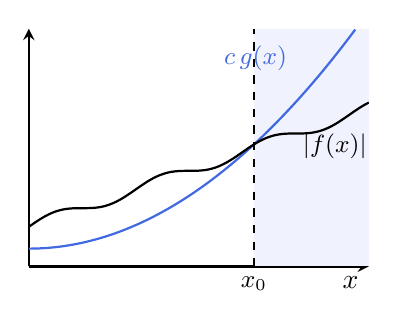
\begin{tikzpicture}
\begin{axis}[boundplot, xlabel={$x$}, ylabel={}]
  \fill[accent!8] (axis cs:6.62,0) rectangle (axis cs:10,12);
  \addplot[accent, domain=0:9.6] {0.9+0.12*x^2};
  \addplot[black, domain=0:10] {2+0.6*x+0.3*sin(deg(2*x))};
  \node[accent, font=\small, left] at (axis cs:7.9,10.5) {$c\,g(x)$};
  \node[font=\small, below] at (axis cs:9,7.2) {$|f(x)|$};
  \draw[dashed] (axis cs:6.62,0) -- (axis cs:6.62,12);
  \node[below, font=\small] at (axis cs:6.62,0) {$x_0$};
\end{axis}
\end{tikzpicture}\\[2pt]
\scriptsize In the shaded region, $|f|$ stays below $c\,g$.
\end{column}
\end{columns}
\end{frame}

\begin{frame}{Simplifying Big-$O$: keep only what matters}
\begin{columns}[T]
\begin{column}{0.47\textwidth}
\begin{block}{Rule 1: drop constant factors}
\begin{itemize}
  \item $O(5x) = O(x)$
  \item $O(c) = O(1)$
  \item $O(c\,f(x)) = O(f(x))$
\end{itemize}
\end{block}
\end{column}
\begin{column}{0.47\textwidth}
\begin{block}{Rule 2: keep only the fastest-growing term}
\begin{itemize}
  \item $3n^2 + 10n + 50 = O(n^2)$
  \item $n + \log n = O(n)$
  \item $2^n + n^{3} = O(2^n)$
\end{itemize}
\end{block}
\end{column}
\end{columns}
\vspace{0.4cm}
\begin{exampleblock}{Why?}
Big-$O$ is about \textbf{large} $n$. There, constants do not change how the work grows, and the fastest-growing term is much bigger than all the others.
\end{exampleblock}
\end{frame}

\begin{frame}{Cheat sheet: common Big-$O$ patterns}
\centering
\footnotesize
\renewcommand{\arraystretch}{1.05}
\begin{tabular}{>{\raggedright\arraybackslash}p{2.9cm} >{\raggedright\arraybackslash}p{4.3cm} c >{\raggedright\arraybackslash}p{3.4cm}}
\toprule
\textbf{code pattern} & \textbf{Python snippet} & \textbf{Big-$O$} & \textbf{example algorithm} \\
\midrule
no loops & \texttt{x = a[5]} & \cbox{green!25}{O(1)} & reading an array element by index \\
halve the input each step & \texttt{while n > 1: n //= 2} & \cbox{green!15}{O(\log n)} & binary search \\
one loop over $n$ items & \texttt{for x in a:}\newline\hspace*{1.2em}\texttt{total += x} & \cbox{yellow!25}{O(n)} & going through an array once \\
repeat a halving loop $n$ times & \texttt{for i in range(n):}\newline\hspace*{1.2em}\texttt{k = n}\newline\hspace*{1.2em}\texttt{while k > 1: k //= 2} & \cbox{orange!20}{O(n \log n)} & merge sort; Python's \texttt{sorted(a)} \\
two nested loops & \texttt{for i in range(n):}\newline\hspace*{1.2em}\texttt{for j in range(n):} & \cbox{red!15}{O(n^2)} & bubble sort; every cell of an $n \times n$ grid \\
try every subset & {\scriptsize\texttt{for k in range(2**n):}} & \cbox{red!35}{O(2^n)} & listing all subsets of a list \\
\bottomrule
\end{tabular}

\vspace{0.1cm}
\scriptsize Green grows slowly, red grows fast. The $n\log n$ row is the $O(n)$ loop around the $O(\log n)$ loop.
\end{frame}

\begin{frame}{Why these growth rates?}
\begin{columns}[T]
\begin{column}{0.31\textwidth}
\centering
\textbf{$O(\log n)$}\\[4pt]
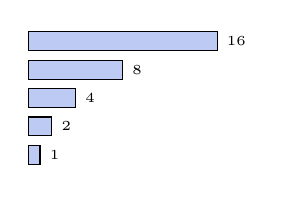
\begin{tikzpicture}[scale=0.6]
  \foreach \w/\y in {16/0, 8/-0.6, 4/-1.2, 2/-1.8, 1/-2.4}{
    \fill[accent!35] (0,\y) rectangle ++(\w*0.25,0.4);
    \draw (0,\y) rectangle ++(\w*0.25,0.4);
    \node[right, font=\tiny] at (\w*0.25,\y+0.2) {\w};
  }
\end{tikzpicture}\\[4pt]
\scriptsize Each step keeps half: 16 items need 4 halvings, $\log_2 16 = 4$.
\end{column}
\begin{column}{0.31\textwidth}
\centering
\textbf{$O(n \log n)$}\\[4pt]
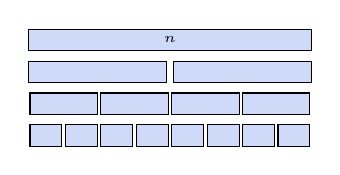
\begin{tikzpicture}[scale=0.45, every node/.style={font=\tiny}]
  \draw[fill=accent!25] (0,0) rectangle (8,0.6); \node at (4,0.3) {$n$};
  \draw[fill=accent!25] (0,-0.9) rectangle (3.9,-0.3); \draw[fill=accent!25] (4.1,-0.9) rectangle (8,-0.3);
  \foreach \i in {0,1,2,3} \draw[fill=accent!25] (\i*2+0.05,-1.8) rectangle (\i*2+1.95,-1.2);
  \foreach \i in {0,...,7} \draw[fill=accent!25] (\i+0.05,-2.7) rectangle (\i+0.95,-2.1);
\end{tikzpicture}\\[4pt]
\scriptsize Merge sort: $\log_2 n$ levels of halving, and combining costs $n$ per level.
\end{column}
\begin{column}{0.31\textwidth}
\centering
\textbf{$O(n^2)$}\\[4pt]
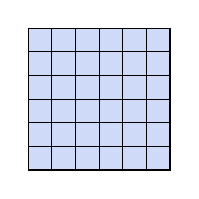
\begin{tikzpicture}[scale=0.3]
  \foreach \i in {0,...,5} \foreach \j in {0,...,5} \draw[fill=accent!25] (\i,\j) rectangle ++(1,1);
\end{tikzpicture}\\[4pt]
\scriptsize Nested loops visit all $n \times n$ pairs: twice the input, four times the work.
\end{column}
\end{columns}
\vspace{0.4cm}
\centering\scriptsize $O(1)$ and $O(n)$ need no picture: a fixed amount of work, or a fixed amount per element.
\end{frame}

\begin{frame}{Proving Big-$O$ vs.\ measuring it}
\begin{columns}[T]
\begin{column}{0.5\textwidth}
\small
\begin{itemize}
  \item Big-$O$ is a statement about \textbf{all} $x \ge x_0$. It is \textbf{proved}: find $c, x_0$ (or use a limit).
  \item Experiments (timings, loglog slopes, the doubling factor) look at \textbf{finitely many} $n$. They can \textbf{check} a prediction, but not prove it.
\end{itemize}
\begin{alertblock}{A measurement that misleads}
\footnotesize
$f(n) = n^2 + 10^6 n$ is $O(n^2)$ and \textbf{not} $O(n)$, yet near $n = 1000$:
\begin{itemize}\footnotesize
  \item doubling factor $f(2n)/f(n) = 2.00$;
  \item loglog slope on $100 \ldots 1600$: $1.00$.
\end{itemize}
Both suggest $O(n)$. The $n^2$ term only wins for $n > 10^6$ (slope $2.0$ near $10^8$).
\end{alertblock}
\end{column}
\begin{column}{0.47\textwidth}
\centering
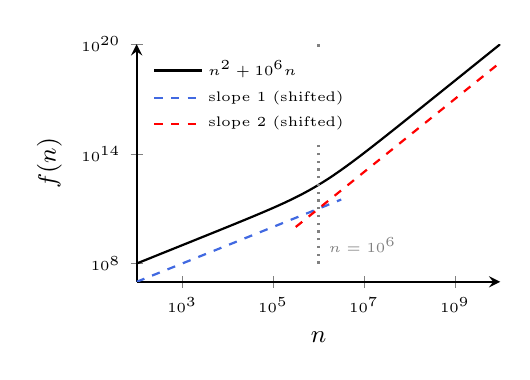
\begin{tikzpicture}
\begin{axis}[width=6.2cm, height=4.6cm, xmode=log, ymode=log, axis lines=left,
  xmin=1e2, xmax=1e10, xlabel={$n$}, ylabel={$f(n)$}, thick,
  tick label style={font=\tiny}, label style={font=\small},
  legend style={font=\tiny, draw=none, at={(0.02,0.98)}, anchor=north west}]
  \addplot[black, domain=2:10, samples=60] ({10^x}, {(10^x)^2 + 1e6*10^x}); \addlegendentry{$n^2 + 10^6 n$}
  \addplot[accent, dashed, domain=2:6.5, samples=10] ({10^x}, {1e5*10^x}); \addlegendentry{slope 1 (shifted)}
  \addplot[red, dashed, domain=5.5:10, samples=10] ({10^x}, {0.1*(10^x)^2}); \addlegendentry{slope 2 (shifted)}
  \draw[gray, dotted] (axis cs:1e6,1e8) -- (axis cs:1e6,1e20);
  \node[gray, font=\tiny, right] at (axis cs:1e6,1e9) {$n = 10^6$};
\end{axis}
\end{tikzpicture}\\[2pt]
\scriptsize The doubling factor is only reliable for polynomial growth, and only once $n$ is large enough: $\log n$ shows up as $+1$, and $2^n$ gives no constant factor at all.
\end{column}
\end{columns}
\end{frame}

\begin{frame}[fragile]{Complexity of an algorithm: \texttt{maximum}}
\begin{columns}[T]
\begin{column}{0.5\textwidth}
\begin{lstlisting}
def maximum(x):
    xmax = -np.inf
    for xi in x:
        if xi > xmax:
            xmax = xi
    return xmax
\end{lstlisting}
\small
\begin{itemize}
  \item One loop over the $n$ entries, constant work per iteration.
  \item \textbf{Time}: $O(n)$. \quad \textbf{Space}: $O(1)$ extra.
\end{itemize}
\scriptsize ``Runs in $O(n^2)$ time'' means: the run time scales, at worst, quadratically with $n$.
\end{column}
\begin{column}{0.47\textwidth}
\small
To \textbf{check} this prediction, time it and plot on \texttt{loglog} axes. If $t(n)$ grows like $n^a$,
\[
t(n) \sim c\,n^{a} \;\Rightarrow\; \log t \sim a \log n + \log c ,
\]
so the \textbf{slope is the exponent} $a$:
\begin{lstlisting}
coeff = np.polyfit(np.log(ns),
                   np.log(ts), 1)
coeff[0]    # estimated exponent
\end{lstlisting}
\end{column}
\end{columns}
\end{frame}

\begin{frame}{Measuring \texttt{maximum} on a \texttt{loglog} plot}
\begin{columns}[c]
\begin{column}{0.5\textwidth}
\centering
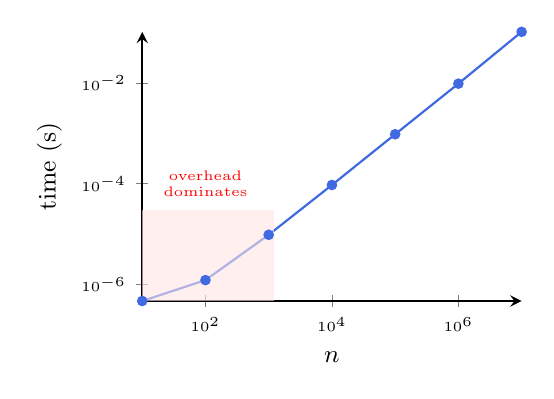
\begin{tikzpicture}
\begin{axis}[width=6.4cm, height=5cm, xmode=log, ymode=log, axis lines=left,
  xlabel={$n$}, ylabel={time (s)}, thick, tick label style={font=\tiny}, label style={font=\small}]
  \addplot[accent, mark=*, mark size=1.5pt] coordinates {(10,4.72e-07) (100,1.225e-06) (1000,9.693e-06) (10000,9.419e-05) (100000,0.0009553) (1e+06,0.009627) (1e+07,0.1026)};
  \fill[red!10, opacity=0.6] (axis cs:8,2e-7) rectangle (axis cs:1.2e3,3e-5);
  \node[red, font=\tiny, align=center] at (axis cs:1e2,1e-4) {overhead\\dominates};
\end{axis}
\end{tikzpicture}
\end{column}
\begin{column}{0.47\textwidth}
\small
\begin{tabular}{lc}
\toprule
fit over & slope \\
\midrule
all $n$ ($10$ to $10^7$) & $0.92$ \\
$n \ge 10^4$ only & $1.01$ \\
\bottomrule
\end{tabular}\\[6pt]
\begin{itemize}
  \item For small $n$ the fixed cost of calling the function dominates, which flattens the curve.
  \item \textbf{Fit only the large-$n$ part.} Then the slope $\approx 1$ \textbf{agrees} with the prediction $O(n)$.
\end{itemize}
\scriptsize (measured in pure Python; your times will differ, the slope should not)
\end{column}
\end{columns}
\end{frame}

\begin{frame}{Exercise: why \texttt{semilogy} for exponential growth?}
\begin{columns}[T]
\begin{column}{0.5\textwidth}
\small
If $t(n) \sim c\, b^{\,n}$, then
\[
\log t(n) \sim n \log b + \log c .
\]
\begin{itemize}
  \item On a \texttt{semilogy} plot this is a \textbf{straight line}; on normal axes the values span many orders of magnitude.
  \item The \textbf{slope} is $\log b$, so $b = e^{\text{slope}}$ is the growth factor per extra element.
\end{itemize}
\end{column}
\begin{column}{0.46\textwidth}
\begin{exampleblock}{Example}
\small If the time \textbf{doubles} with each extra element, $t(n) \sim c\,2^{n}$: the \texttt{semilogy} plot is a straight line with slope $\log 2 \approx 0.69$, and $e^{0.69} = 2$ recovers the factor.
\end{exampleblock}
\scriptsize Compare: polynomial $\Rightarrow$ \texttt{loglog}, slope = exponent. Exponential $\Rightarrow$ \texttt{semilogy}, slope = $\log b$.
\end{column}
\end{columns}
\end{frame}

% ============================================================
\section{Convergence of algorithms}
% ============================================================

\begin{frame}{Convergence of algorithms}
\begin{columns}[T]
\begin{column}{0.52\textwidth}
\small
Many numerical algorithms produce better and better approximations $x_k$ of a true solution $x_\ast$. The \textbf{error} is
\[
\epsilon_k = |x_k - x_\ast| ,
\]
and the algorithm \textbf{converges} if $\displaystyle\lim_{k\to\infty} \epsilon_k = 0$.
\vspace{0.1cm}
\begin{block}{Our goals}
not to prove convergence, but to \textbf{verify} it, \textbf{measure its rate}, and \textbf{compare} algorithms using experimental data.
\end{block}
\end{column}
\begin{column}{0.45\textwidth}
\small
In practice $x_\ast$ is \textbf{unknown}. Two substitutes:
\begin{itemize}
  \item run $N$ iterations and use $\tilde\epsilon_k = |x_k - x_N|$;
  \item monitor the change $\delta_k = |x_k - x_{k-1}|$ and \textbf{stop} when it is small enough.
\end{itemize}
\vspace{0.1cm}
\begin{alertblock}{Floating point floor}
\scriptsize $\delta_k$ cannot drop below about $\varepsilon\,|x_k| \approx 10^{-16}|x_k|$: never ask for a smaller tolerance, and always cap the number of iterations.
\end{alertblock}
\end{column}
\end{columns}
\end{frame}

\begin{frame}{Rate of convergence: how fast does the error shrink?}
\small
The key question: \textbf{by how much does one iteration shrink the error?}
\vspace{0.15cm}
\begin{center}
\footnotesize
\renewcommand{\arraystretch}{1.2}
\begin{tabular}{>{\raggedright\arraybackslash}p{1.8cm} >{\raggedright\arraybackslash}p{4.3cm} >{\raggedright\arraybackslash}p{3.4cm} c}
\toprule
\textbf{name} & \textbf{each iteration \ldots} & \textbf{example errors} & \textbf{to reach $10^{-6}$} \\
\midrule
\textbf{sublinear} & shrinks the error by less and less: $\epsilon_{k+1}/\epsilon_k \to 1$ & $\epsilon_k = 1/k$:\newline $1,\ 0.5,\ 0.33,\ 0.25,\ \ldots$ & $10^{6}$ iterations \\
\textbf{linear} & shrinks the error by the \textbf{same factor} $C < 1$: $\epsilon_{k+1} \approx C\,\epsilon_k$ & $C = 0.5$:\newline $1,\ 0.5,\ 0.25,\ 0.125,\ \ldots$ & $20$ iterations \\
\textbf{quadratic} & \textbf{squares} the error, so the correct digits double: $\epsilon_{k+1} \approx C\,\epsilon_k^{2}$ & $10^{-1},\ 10^{-2},\ 10^{-4},\ 10^{-8}$ & $3$ iterations \\
\bottomrule
\end{tabular}
\end{center}
\vspace{0.1cm}
\begin{block}{The order $q$ (precise definition)}
\footnotesize The convergence has order $q$ if $\epsilon_{k+1} / \epsilon_k^{\,q} \to C$ with $0 < C < \infty$. \quad
Linear and sublinear both have $q = 1$ (only $C$ differs: $C < 1$ vs.\ $C = 1$); quadratic has $q = 2$; any $q > 1$ is called \textbf{superlinear}.
\end{block}
\end{frame}

\begin{frame}{Measuring the rate: \texttt{semilogy} of the error}
\begin{columns}[c]
\begin{column}{0.45\textwidth}
\small
Taking logarithms of $\epsilon_{k+1} \approx C\,\epsilon_k^{\,q}$:
\[
\log \epsilon_{k+1} - q \log \epsilon_k \approx \log C .
\]
\begin{itemize}
  \item $q = 1$: $\log \epsilon_k$ is a \textbf{straight line} with slope $\log C$.
  \item $q > 1$: $\log \epsilon_k \to -\infty$ at an \textbf{exponential} rate: the curve bends down.
  \item sublinear: the curve \textbf{flattens}.
\end{itemize}
\scriptsize Look at large enough $k$: the asymptotic behaviour may take many iterations to appear.
\end{column}
\begin{column}{0.53\textwidth}
\centering
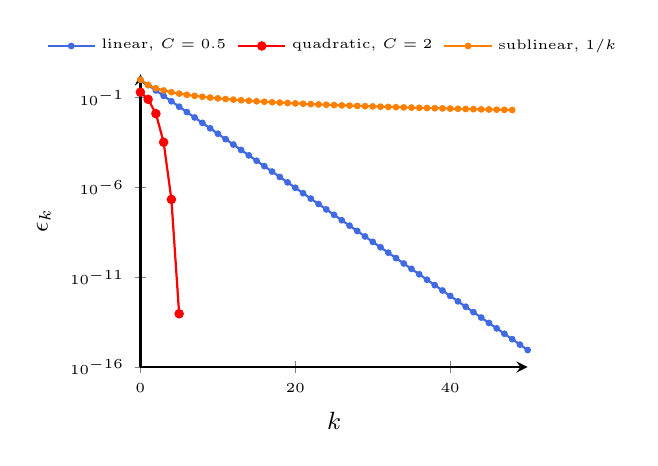
\begin{tikzpicture}
\begin{axis}[width=6.5cm, height=5.3cm, ymode=log, axis lines=left,
  xmin=0, xmax=50, ymin=1e-16, ymax=2, xlabel={$k$}, ylabel={$\epsilon_k$}, thick,
  tick label style={font=\tiny}, label style={font=\small}, legend columns=3, legend style={/tikz/every even column/.append style={column sep=2pt}},
  legend style={font=\tiny, draw=none, at={(0.5,1.03)}, anchor=south}]
  \addplot[accent, mark=*, mark size=0.8pt] coordinates {(0,1) (1,0.5) (2,0.25) (3,0.125) (4,0.0625) (5,0.03125) (6,0.01562) (7,0.007812) (8,0.003906) (9,0.001953) (10,0.0009766) (11,0.0004883) (12,0.0002441) (13,0.0001221) (14,6.104e-05) (15,3.052e-05) (16,1.526e-05) (17,7.629e-06) (18,3.815e-06) (19,1.907e-06) (20,9.537e-07) (21,4.768e-07) (22,2.384e-07) (23,1.192e-07) (24,5.96e-08) (25,2.98e-08) (26,1.49e-08) (27,7.451e-09) (28,3.725e-09) (29,1.863e-09) (30,9.313e-10) (31,4.657e-10) (32,2.328e-10) (33,1.164e-10) (34,5.821e-11) (35,2.91e-11) (36,1.455e-11) (37,7.276e-12) (38,3.638e-12) (39,1.819e-12) (40,9.095e-13) (41,4.547e-13) (42,2.274e-13) (43,1.137e-13) (44,5.684e-14) (45,2.842e-14) (46,1.421e-14) (47,7.105e-15) (48,3.553e-15) (49,1.776e-15) (50,8.882e-16)}; \addlegendentry{linear, $C = 0.5$}
  \addplot[red, mark=*, mark size=1.3pt] coordinates {(0,0.2) (1,0.08) (2,0.0128) (3,0.0003277) (4,2.147e-07) (5,9.223e-14)}; \addlegendentry{quadratic, $C = 2$}
  \addplot[orange, mark=*, mark size=0.8pt] coordinates {(0,1) (1,0.5) (2,0.3333) (3,0.25) (4,0.2) (5,0.1667) (6,0.1429) (7,0.125) (8,0.1111) (9,0.1) (10,0.09091) (11,0.08333) (12,0.07692) (13,0.07143) (14,0.06667) (15,0.0625) (16,0.05882) (17,0.05556) (18,0.05263) (19,0.05) (20,0.04762) (21,0.04545) (22,0.04348) (23,0.04167) (24,0.04) (25,0.03846) (26,0.03704) (27,0.03571) (28,0.03448) (29,0.03333) (30,0.03226) (31,0.03125) (32,0.0303) (33,0.02941) (34,0.02857) (35,0.02778) (36,0.02703) (37,0.02632) (38,0.02564) (39,0.025) (40,0.02439) (41,0.02381) (42,0.02326) (43,0.02273) (44,0.02222) (45,0.02174) (46,0.02128) (47,0.02083) (48,0.02041)}; \addlegendentry{sublinear, $1/k$}
\end{axis}
\end{tikzpicture}
\end{column}
\end{columns}
\end{frame}

\begin{frame}[fragile]{Estimating $q$ from data}
\begin{columns}[T]
\begin{column}{0.54\textwidth}
\small
Asymptotically $\epsilon_{k+1} \approx C \epsilon_k^q$. With $\ell_k = \log \epsilon_k$:
\[
\ell_{k+1} \approx \log C + q\,\ell_k .
\]
Subtracting consecutive steps cancels $C$: the differences
$d_k = \ell_{k+1} - \ell_k$ satisfy
\[
d_{k+1} \approx q\, d_k \quad\Longrightarrow\quad d_k \approx d_0\, q^k .
\]
So $k$ enters through $q^k$, and one more log makes it linear:
\[
\begin{aligned}
\log\bigl|\log(\epsilon_{k+1}/\epsilon_k)\bigr|
  &= \log\bigl|\log \epsilon_{k+1} - \log \epsilon_k\bigr| \\
  &= \log|d_k| \approx \log|d_0| + k \log q ,
\end{aligned}
\]
a line in $k$ with \textbf{slope $\log q$}.
\end{column}

\begin{column}{0.44\textwidth}
\begin{lstlisting}[basicstyle=\ttfamily\scriptsize]
def estimate_q(eps):
    d = np.diff(np.log(eps))
    y = np.log(np.abs(d))
    x = np.arange(len(y))
    line = np.polyfit(x, y, 1)
    return np.exp(line[0])
\end{lstlisting}

\vspace{4pt}
{\centering
\small
\begin{tabular}{lc}
\toprule
sequence & estimated $q$ \\
\midrule
sublinear $1/k$ & $<1.0$ \\
linear ($C = 0.5$) & $1.00$ \\
quadratic ($C = 2$) & $2.00$ \\
\bottomrule
\end{tabular}\par}
\vspace{6pt}

\scriptsize A rough but easy estimate: it fits a line through \emph{all} the points, including the early, non-asymptotic ones.
\end{column}
\end{columns}
\end{frame}

\begin{frame}{Exercise 2: the sublinear estimate depends on the length}
\begin{columns}[T]
\begin{column}{0.45\textwidth}
\centering
\small
$\epsilon_k = 1/k$, \ $k = 1, \ldots, n-1$:\\[4pt]
\begin{tabular}{rc}
\toprule
length $n$ & estimated $q$ \\
\midrule
$50$ & $0.9466$ \\
$100$ & $0.9720$ \\
$500$ & $0.9941$ \\
$1000$ & $0.9970$ \\
$5000$ & $0.9994$ \\
$10000$ & $0.9997$ \\
\bottomrule
\end{tabular}
\end{column}
\begin{column}{0.52\textwidth}
\small
\begin{itemize}
  \item The estimate approaches $q = 1$ as the sequence gets longer: sublinear convergence has $q = 1$ with $C = 1$.
  \item Short sequences are dominated by the early terms, where $\epsilon_{k+1}/\epsilon_k$ is still far from its limit.
\end{itemize}
\begin{exampleblock}{Same lesson as for Big-$O$}
\scriptsize An estimate from finitely many data points describes the asymptotic behaviour only once $k$ (or $n$) is large enough.
\end{exampleblock}
\end{column}
\end{columns}
\end{frame}

\begin{frame}{Real algorithms: fixed point vs.\ Newton}
\begin{columns}[c]
\begin{column}{0.42\textwidth}
\small
Errors $\epsilon_k$ of three real sequences:
\begin{itemize}
  \item \textbf{linear} ($\cos$ iteration): a straight line, slope $\log C$ with $C \approx 0.67$;
  \item \textbf{quadratic} (Newton for $\sqrt 2$): bends down;
  \item \textbf{sublinear} ($(1+1/k)^k \to e$): flattens out.
\end{itemize}
\vspace{0.2cm}
\begin{alertblock}{The floor}
Newton reaches $\approx 10^{-16}$ in 5 iterations and cannot go lower: that is machine epsilon.
\end{alertblock}
\end{column}
\begin{column}{0.56\textwidth}
\centering
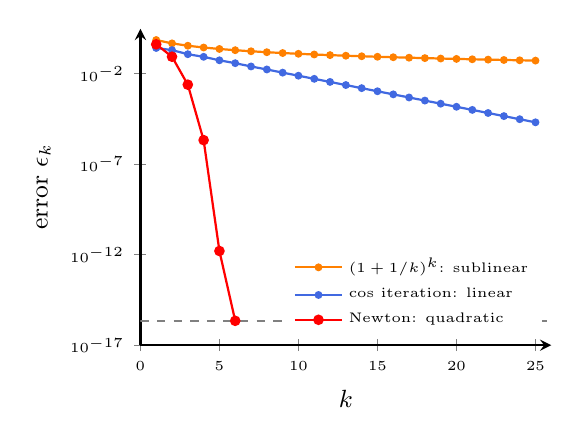
\begin{tikzpicture}
\begin{axis}[width=6.8cm, height=5.6cm, ymode=log, axis lines=left,
  xmin=0, xmax=26, ymin=1e-17, ymax=3, xlabel={$k$}, ylabel={error $\epsilon_k$},
  thick, tick label style={font=\tiny}, label style={font=\small},
  legend style={font=\tiny, draw=none, at={(0.98,0.02)}, anchor=south east}]
  \addplot[orange, mark=*, mark size=1pt] coordinates {(1,0.7183) (2,0.4683) (3,0.3479) (4,0.2769) (5,0.23) (6,0.1967) (7,0.1718) (8,0.1525) (9,0.1371) (10,0.1245) (11,0.1141) (12,0.1052) (13,0.09768) (14,0.09113) (15,0.0854) (16,0.08035) (17,0.07587) (18,0.07186) (19,0.06825) (20,0.06498) (21,0.06202) (22,0.05931) (23,0.05683) (24,0.05455) (25,0.05245)};
  \addlegendentry{$(1+1/k)^k$: sublinear}
  \addplot[accent, mark=*, mark size=1pt] coordinates {(1,0.2609) (2,0.1988) (3,0.1185) (4,0.0848) (5,0.0544) (6,0.03772) (7,0.02487) (8,0.01698) (9,0.01133) (10,0.007681) (11,0.005152) (12,0.00348) (13,0.00234) (14,0.001578) (15,0.001062) (16,0.0007159) (17,0.0004821) (18,0.0003248) (19,0.0002188) (20,0.0001474) (21,9.927e-05) (22,6.687e-05) (23,4.504e-05) (24,3.034e-05) (25,2.044e-05)};
  \addlegendentry{$\cos$ iteration: linear}
  \addplot[red, mark=*, mark size=1.5pt] coordinates {(1,0.4142) (2,0.08579) (3,0.002453) (4,2.124e-06) (5,1.595e-12) (6,2.22e-16)};
  \addlegendentry{Newton: quadratic}
  \draw[gray, dashed] (axis cs:0,2.2e-16) -- (axis cs:26,2.2e-16);
  \node[gray, font=\tiny, above] at (axis cs:20,2.2e-16) {machine epsilon};
\end{axis}
\end{tikzpicture}
\end{column}
\end{columns}
\end{frame}

% ============================================================
\section{Summary}
% ============================================================

\begin{frame}{Summary}
\begin{columns}[T]
\begin{column}{0.48\textwidth}
\begin{block}{Big-$O$}
\footnotesize
\begin{itemize}
  \item $f = O(g)$: $f$ grows no faster than $g$ (an upper bound).
  \item \textbf{Prove} with witnesses $c, x_0$; drop constants and smaller terms.
  \item Cheat sheet: $1 \ll \log n \ll n \ll n\log n \ll n^2 \ll 2^n$.
  \item \textbf{Check} (not prove) with experiments: \texttt{loglog} slope for polynomials, \texttt{semilogy} for exponentials; fit only large $n$.
\end{itemize}
\end{block}
\end{column}
\begin{column}{0.48\textwidth}
\begin{block}{Convergence}
\footnotesize
\begin{itemize}
  \item Error $\epsilon_k = |x_k - x_\ast| \to 0$; stop when $\delta_k = |x_k - x_{k-1}|$ is small.
  \item Order $q$: linear ($q = 1$, $C < 1$), sublinear, superlinear, quadratic ($q = 2$).
  \item \texttt{semilogy} of $\epsilon_k$: line = linear, bends down = superlinear.
  \item Floating point sets a floor near $10^{-16}$.
\end{itemize}
\end{block}
\end{column}
\end{columns}

\end{frame}

\end{document}
